
% Mayan Ascendancy chapter --------------------------------------------
\chapter*{Mayan Ascendancy}
\addcontentsline{toc}{chapter}{Mayan Ascendancy}

\begin{flushright}
\parbox{0.8\textwidth}{
\emph{The world has achieved brilliance without wisdom, power without
conscience. Our is a world of nuclear giants and ethical infants. \\
\hspace*{\fill}{\textperiodcentered \textperiodcentered \textperiodcentered \hspace*{0.2em} Omar Nelson Bradley} } }
\end{flushright}

\noindent
Mayan Ascendancy is chess variant which is played on 12 x 12 board with
yellow and blue fields and with dark yellow and dark blue pieces. In
algebraic notation, columns are enumerated from 'a' to 'l', and rows are
enumerated from '1' to '12'. A new piece is introduced, Pyramid.

\clearpage % ..........................................................

\section*{Pyramid}
\addcontentsline{toc}{section}{Pyramid}

\noindent
\begin{wrapfigure}[12]{l}{0.4\textwidth}
\centering
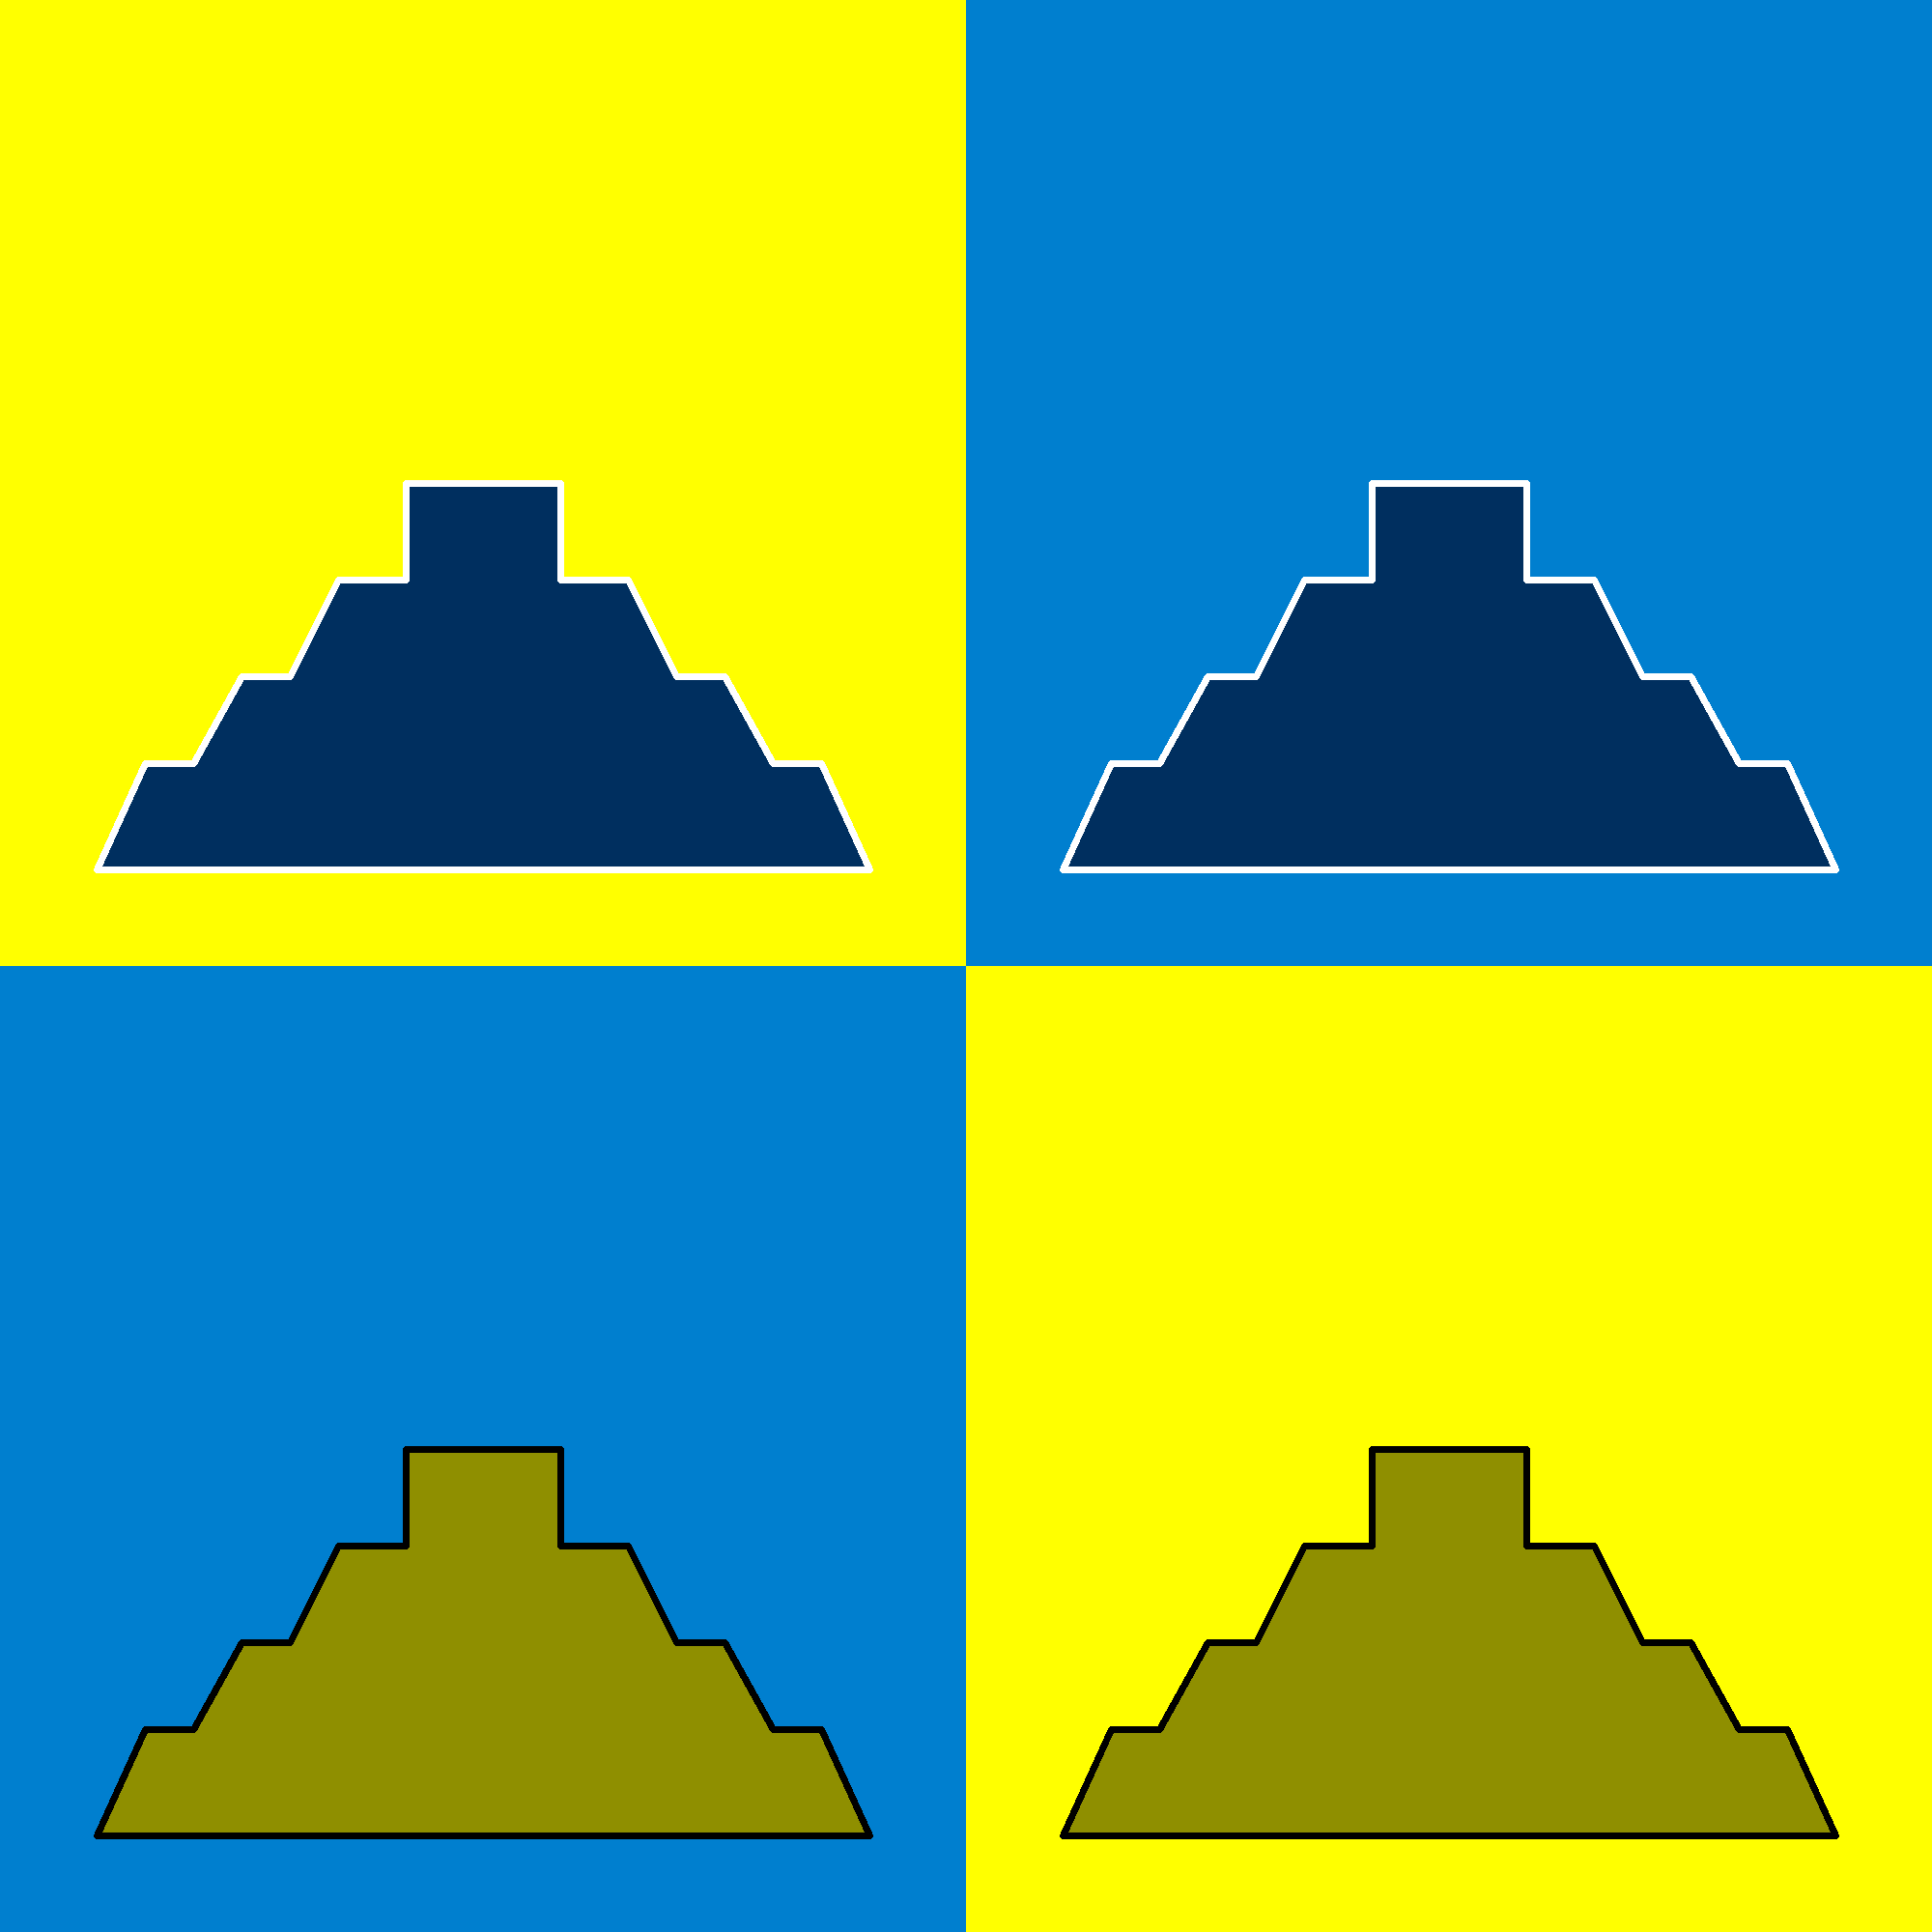
\includegraphics[width=0.4\textwidth, keepaspectratio=true]{pieces/08_pyramid.png}
\caption{Pyramid}
\label{fig:08_pyramid}
\end{wrapfigure}
Pyramid is passive piece, meaning it can't move on its' own, it has to be
activated first. This is done by capturing a field at which Pyramid stands
with own other piece and then move Pyramid further.

Once activated Pyramid moves similar to Rook, only real difference is that
it can move for only so many fields as piece activating it has moved, i.e.
for at most as momentum received.

\subsection*{Momentum}
\addcontentsline{toc}{subsection}{Momentum}

Momentum is count of step-fields traveled over by a piece. Pyramid receives
momentum from piece which activates it. Momentum is spent by Pyramid when
moving, one for each step-field travelled. So Pyramid can't move for more
fields than received momentum, i.e. for more than activating piece has
travelled. Momentum can't be saved for later, it is wasted when Pyramid
moves for less than received momentum.

\clearpage % ..........................................................

\subsection*{Pyramid (cont.)}
\addcontentsline{toc}{subsection}{Pyramid (cont.)}

Pyramid can't check opponent's King, and consequently can't contribute to
checkmate. Pyramid can capture all the other opponent's pieces after it has
been activated, even if it has no remaining momentum, i.e. can't move any
further.

Pyramid can also promote own Pawns on opponen't side of the board. It can
also convert any opponent's piece, except King, on own side of the board.
To do either of these things, Pyramid does not have to have any remaining
momentum, it's enough if piece in question is within reach.

Pyramid can also activate other Pyramid, and transfer remaining momentum to it.
There has to be remaining momentum, it must be greater than 0 for activation
to be permitted.

In algebraic notation symbol for Pyramid is 'A', to avoid confusion with Pawn.

\clearpage % ..........................................................

\subsection*{Activation}
\addcontentsline{toc}{subsection}{Activation}

\noindent
\begin{figure}[!h]
% \begin{figure}[!t]
\includegraphics[width=1.0\textwidth, keepaspectratio=true]{examples/06_ma/scn_ma_01_pyramid_activation_init.png}
\caption{Pyramid activation}
\label{fig:scn_ma_01_pyramid_activation_init}
% \centering
\end{figure}

Here Pegasus is about to capture field on which Pyramid stands. Note, only
step-fields are counted towards momentum. After activation Pyramid would be
limited to move at most 4 fields across, i.e. at most the momentum it received
from Pegasus.

\clearpage % ..........................................................

\noindent
\begin{figure}[!h]
% \begin{figure}[!t]
\includegraphics[width=1.0\textwidth, keepaspectratio=true]{examples/06_ma/scn_ma_02_pyramid_activated.png}
\caption{Pyramid activated}
\label{fig:scn_ma_02_pyramid_activated}
% \centering
\end{figure}

Above, arrows show all possible moves by Pyramid. Just like Rook, Pyramid has to
stop before own Bishop. Pyramid can capture opponent's Knight, but can't move any
further after capture. Pyramid can also capture opponent's Bishop, despite being
barely reachable.

\clearpage % ..........................................................

\noindent
\begin{figure}[!h]
% \begin{figure}[!t]
\includegraphics[width=1.0\textwidth, keepaspectratio=true]{examples/06_ma/scn_ma_03_pyramid_activation_end.png}
\caption{Pyramid activation end}
\label{fig:scn_ma_03_pyramid_activation_end}
% \centering
\end{figure}

Here, Pyramid movement ends by capturing opponent's Knight, which also ends light
player's complete move.

\clearpage % ..........................................................

\subsection*{Promotion}
\addcontentsline{toc}{subsection}{Promotion}

Pyramid can promote own Pawns, but only on opponent's side of the board.
Promotion is done by activating Pyramid which then marks Pawn for promotion
by touching either Pawn or field at which it stands. Pyramid then leaves
board as if it was captured, and Pawn is replaced by desired piece, for
instance Queen.

Both Pyramid and Pawn in question has to reside on opponent's side of the
board before promotion can take place. Piece which activates Pyramid need
not to be on opponent's side of the board.

Piece which Pawn can be promoted to is from the set of all starting pieces,
except King. This promoting-to piece is not limited to pieces already being
captured.

\clearpage % ..........................................................

\noindent
\begin{figure}[!h]
% \begin{figure}[!t]
\includegraphics[width=1.0\textwidth, keepaspectratio=true]{examples/06_ma/scn_ma_05_promo_init.png}
\caption{Promotion start}
\label{fig:scn_ma_05_promo_init}
% \centering
\end{figure}

Here, Pegasus is accumulating momentum while travelling over step-fields. After
activation Pyramid would be limited to move at most 4 fields across, i.e. at most
the momentum it received from Pegasus.

\clearpage % ..........................................................

\noindent
\begin{figure}[!h]
% \begin{figure}[!t]
\includegraphics[width=1.0\textwidth, keepaspectratio=true]{examples/06_ma/scn_ma_06_promo_pyramid_activated.png}
\caption{Promotion, Pyramid activated}
\label{fig:scn_ma_06_promo_pyramid_activated}
% \centering
\end{figure}

Above, Pegasus captured field at which Pyramid was situated, arrows now show
all possible moves by Pyramid. Pyramid can't promote Pawn 2, as it is still
located on own half of the chessboard. Just as Rook, Pyramid can't advance
past Pawn 2. Only full movement to the right leads to promotion of Pawn 1,
shown in blue.

\clearpage % ..........................................................

\noindent
\begin{figure}[!h]
% \begin{figure}[!t]
\includegraphics[width=1.0\textwidth, keepaspectratio=true]{examples/06_ma/scn_ma_07_promo_end.png}
\caption{Promotion end}
\label{fig:scn_ma_07_promo_end}
% \centering
\end{figure}

Now that Pyramid has reached Pawn 1, it is removed from the board and piece of
choice, in this instance Queen, replaces Pawn. Just as with ordinary promotion,
this can take place regardless of which pieces has been captured, e.g. even if
own Queen is still present on chessboard.

\clearpage % ..........................................................

\subsection*{Conversion}
\addcontentsline{toc}{subsection}{Conversion}

Pyramid can convert opponent's pieces, except King, but only on own side of
the board. Conversion is done by activating Pyramid which then marks opponent's
piece for conversion by touching either piece or field at which it stands. Now
Pyramid leaves the board as if it was captured, and opponent's piece is replaced
by own piece of the same type.

Both Pyramid and opponent's piece has to reside on own side of the board
before conversion can take place. Piece which activates Pyramid need not
to be on own side of the board. As with promotion, conversion is not limited
to pieces which has been captured.

Note that Pyramid might just as well capture opponent's piece. Differences are
who leaves chessboard, and what remains on captured field. Capture itself with
Pyramid is in no way different than that with Rook. In either case, converting
or capturing, it is enough if Pyramid can reach opponent's piece, i.e. has
enough momentum from activating piece.

\clearpage % ..........................................................

\noindent
\begin{figure}[!h]
% \begin{figure}[!t]
\includegraphics[width=1.0\textwidth, keepaspectratio=true]{examples/06_ma/scn_ma_08_conversion_init.png}
\caption{Conversion start}
\label{fig:scn_ma_08_conversion_init}
% \centering
\end{figure}

For classic pieces, step-fields are just fields which piece traveled over,
in case of Bishop above that is 4 fields. Again, that is momentum Pyramid
will receive with activation and limits how far it could move afterwards.

\clearpage % ..........................................................

\noindent
\begin{figure}[!h]
% \begin{figure}[!t]
\includegraphics[width=1.0\textwidth, keepaspectratio=true]{examples/06_ma/scn_ma_09_conversion_pyramid_activated.png}
\caption{Conversion, Pyramid activated}
\label{fig:scn_ma_09_conversion_pyramid_activated}
% \centering
\end{figure}

Above, Bishop captured field at which Pyramid was situated, arrows now show
all possible moves by Pyramid. Pyramid can't convert opponent's Bishop, as it
is still located on own side of chessboard. Again, just like Rook, Pyramid
can't advance past opponent's Bishop. Only full movement to the right leads
to conversion of opponent's Rook, shown in blue.

\clearpage % ..........................................................

\noindent
\begin{figure}[!h]
% \begin{figure}[!t]
\includegraphics[width=1.0\textwidth, keepaspectratio=true]{examples/06_ma/scn_ma_10_conversion_end.png}
\caption{Conversion end}
\label{fig:scn_ma_10_conversion_end}
% \centering
\end{figure}

Now that Pyramid has reached opponent's Rook, it is removed from the board and
own Rook replaces opponent's Rook. This conversion can still take place, regardless
if any light Rook has been captured or not, i.e. even with both light Rooks still
present on chessboard. Capturing opponent's Rook would simply leave Pyramid in
place of it.

\clearpage % ..........................................................

\subsubsection*{Converting opponent's Rook}
\addcontentsline{toc}{subsubsection}{Converting opponent's Rook}

\noindent
\begin{figure}[!h]
% \begin{figure}[!t]
\includegraphics[width=1.0\textwidth, keepaspectratio=true]{examples/06_ma/scn_ma_11_convert_rook_castling_init.png}
\caption{Converting opponent's Rook}
\label{fig:scn_ma_11_convert_rook_castling_init}
% \centering
\end{figure}

Converting opponent's Rook in an initial position of own Rook grants them ability
to castle.

\noindent
\begin{figure}[!h]
% \begin{figure}[!t]
\includegraphics[width=1.0\textwidth, keepaspectratio=true]{examples/06_ma/scn_ma_12_convert_rook_castling_end.png}
\caption{Possible castling fields}
\label{fig:scn_ma_12_convert_rook_castling_end}
% \centering
\end{figure}

King can now castle to any numbered field. Rook would be moved onto the inner field,
next to the King.

\noindent
\begin{figure}[!h]
% \begin{figure}[!t]
\includegraphics[width=1.0\textwidth, keepaspectratio=true]{examples/06_ma/scn_ma_13_convert_rook_castling.png}
\caption{Castling performed}
\label{fig:scn_ma_13_convert_rook_castling}
% \centering
\end{figure}

To actually perform castling, in the next move or at some point later, all the other
requirements for castling has to be satisfied, with Rook prohibited to move after
conversion.

\clearpage % ..........................................................

\subsubsection*{Converting opponent's Pawn}
\addcontentsline{toc}{subsubsection}{Converting opponent's Pawn}

\noindent
\begin{wrapfigure}[8]{l}{0.6\textwidth}
\centering
\includegraphics[width=0.25\textwidth, keepaspectratio=true]{examples/06_ma/scn_ma_14_convert_pawn_rush_init.png}
\caption{Converting opponent's Pawn}
\label{fig:scn_ma_14_convert_pawn_rush_init}
\end{wrapfigure}
Converting opponent's Pawn in an initial position of own Pawn grants them
ability to be rushed, and subjects them to opponent's en-passant move.

\vspace*{0.2\textheight}
\noindent
\begin{wrapfigure}{l}{0.6\textwidth}
\centering
\includegraphics[width=0.25\textwidth, keepaspectratio=true]{examples/06_ma/scn_ma_15_convert_pawn_rush_end.png}
\caption{Possible initial movement}
\label{fig:scn_ma_15_convert_pawn_rush_end}
\end{wrapfigure}
In this example dark Pawn would have en passant opportunity, should converted
light Pawn be rushed to any numbered field.

\clearpage % ..........................................................

\subsection*{Cascading}
\addcontentsline{toc}{subsection}{Cascading}

\noindent
\begin{figure}[!h]
% \begin{figure}[!t]
\includegraphics[width=1.0\textwidth, keepaspectratio=true]{examples/06_ma/scn_ma_16_cascading_init.png}
\caption{Cascading start}
\label{fig:scn_ma_16_cascading_init}
% \centering
\end{figure}

Once activated, Pyramid can also activate another Pyramid. To do so, activated
Pyramid has to have at least 1 remaining momentum to transfer it to another
Pyramid. If all momentum received was spent moving, Pyramid cannot activate
another Pyramid.

\clearpage % ..........................................................

\noindent
\begin{figure}[!h]
% \begin{figure}[!t]
\includegraphics[width=1.0\textwidth, keepaspectratio=true]{examples/06_ma/scn_ma_17_cascading_pyramid_1_activated.png}
\caption{Cascading, 1st Pyramid activated}
\label{fig:scn_ma_17_cascading_pyramid_1_activated}
% \centering
\end{figure}

Pyramid 1 has been activated by Queen and received momentum of 5, arrows now show
its' all possible moves. Note, Pyramid 3 can't be activated, it's on the very end
of fields reachable by Pyramid 1.

\clearpage % ..........................................................

\noindent
\begin{figure}[!h]
% \begin{figure}[!t]
\includegraphics[width=1.0\textwidth, keepaspectratio=true]{examples/06_ma/scn_ma_18_cascading_pyramid_2_activated.png}
\caption{Cascading, 2nd Pyramid activated}
\label{fig:scn_ma_18_cascading_pyramid_2_activated}
% \centering
\end{figure}

Pyramid 2 has been activated by Pyramid 1 and in the process received momentum of 2,
arrows now show all possible moves by Pyramid 2.

\clearpage % ..........................................................

\noindent
\begin{figure}[!h]
% \begin{figure}[!t]
\includegraphics[width=1.0\textwidth, keepaspectratio=true]{examples/06_ma/scn_ma_19_cascading_end.png}
\caption{Cascading end}
\label{fig:scn_ma_19_cascading_end}
% \centering
\end{figure}

Pyramid 2 has finished its' movement, and so it ends light player's complete move.

\clearpage % ..........................................................

\subsection*{Against King}
\addcontentsline{toc}{subsection}{Against King}

Pyramid can't check opponent's King, meaning that King is not under attack
even if Pyramid could capture any other piece on the same field.

\noindent
\begin{figure}[!h]
% \begin{figure}[!t]
\includegraphics[width=1.0\textwidth, keepaspectratio=true]{examples/06_ma/scn_ma_20_pyramid_vs_king.png}
\caption{Pyramid vs. King}
\label{fig:scn_ma_20_pyramid_vs_king}
% \centering
\end{figure}

Above, King is not under attack from Pyramid.

\noindent
\begin{figure}[!h]
% \begin{figure}[!t]
\includegraphics[width=1.0\textwidth, keepaspectratio=true]{examples/06_ma/scn_ma_21_pyramid_vs_bishop.png}
\caption{Pyramid vs. Bishop}
\label{fig:scn_ma_21_pyramid_vs_bishop}
% \centering
\end{figure}

Bishop in the same place, however, could be captured without any hindrance.

\clearpage % ..........................................................

\subsection*{Activation by Pawn}
\addcontentsline{toc}{subsection}{Activation by Pawn}

\noindent
\begin{figure}[!h]
% \begin{figure}[!t]
\includegraphics[width=1.0\textwidth, keepaspectratio=true]{examples/06_ma/scn_ma_04_pyramid_activation_by_pawn.png}
\caption{Pyramid activation by Pawns}
\label{fig:scn_ma_04_pyramid_activation_by_pawn}
% \centering
\end{figure}

Pawns can activate Pyramid on own capture-field giving it 1 momentum, see Pawn 1.
Pawns can't activate Pyramids on step-fields, and are blocked from moving further,
see Pawns 2 and 3.

\clearpage % ..........................................................

\section*{En passant}
\addcontentsline{toc}{section}{En passant}

\noindent
\begin{wrapfigure}{l}{0.4\textwidth}
\centering
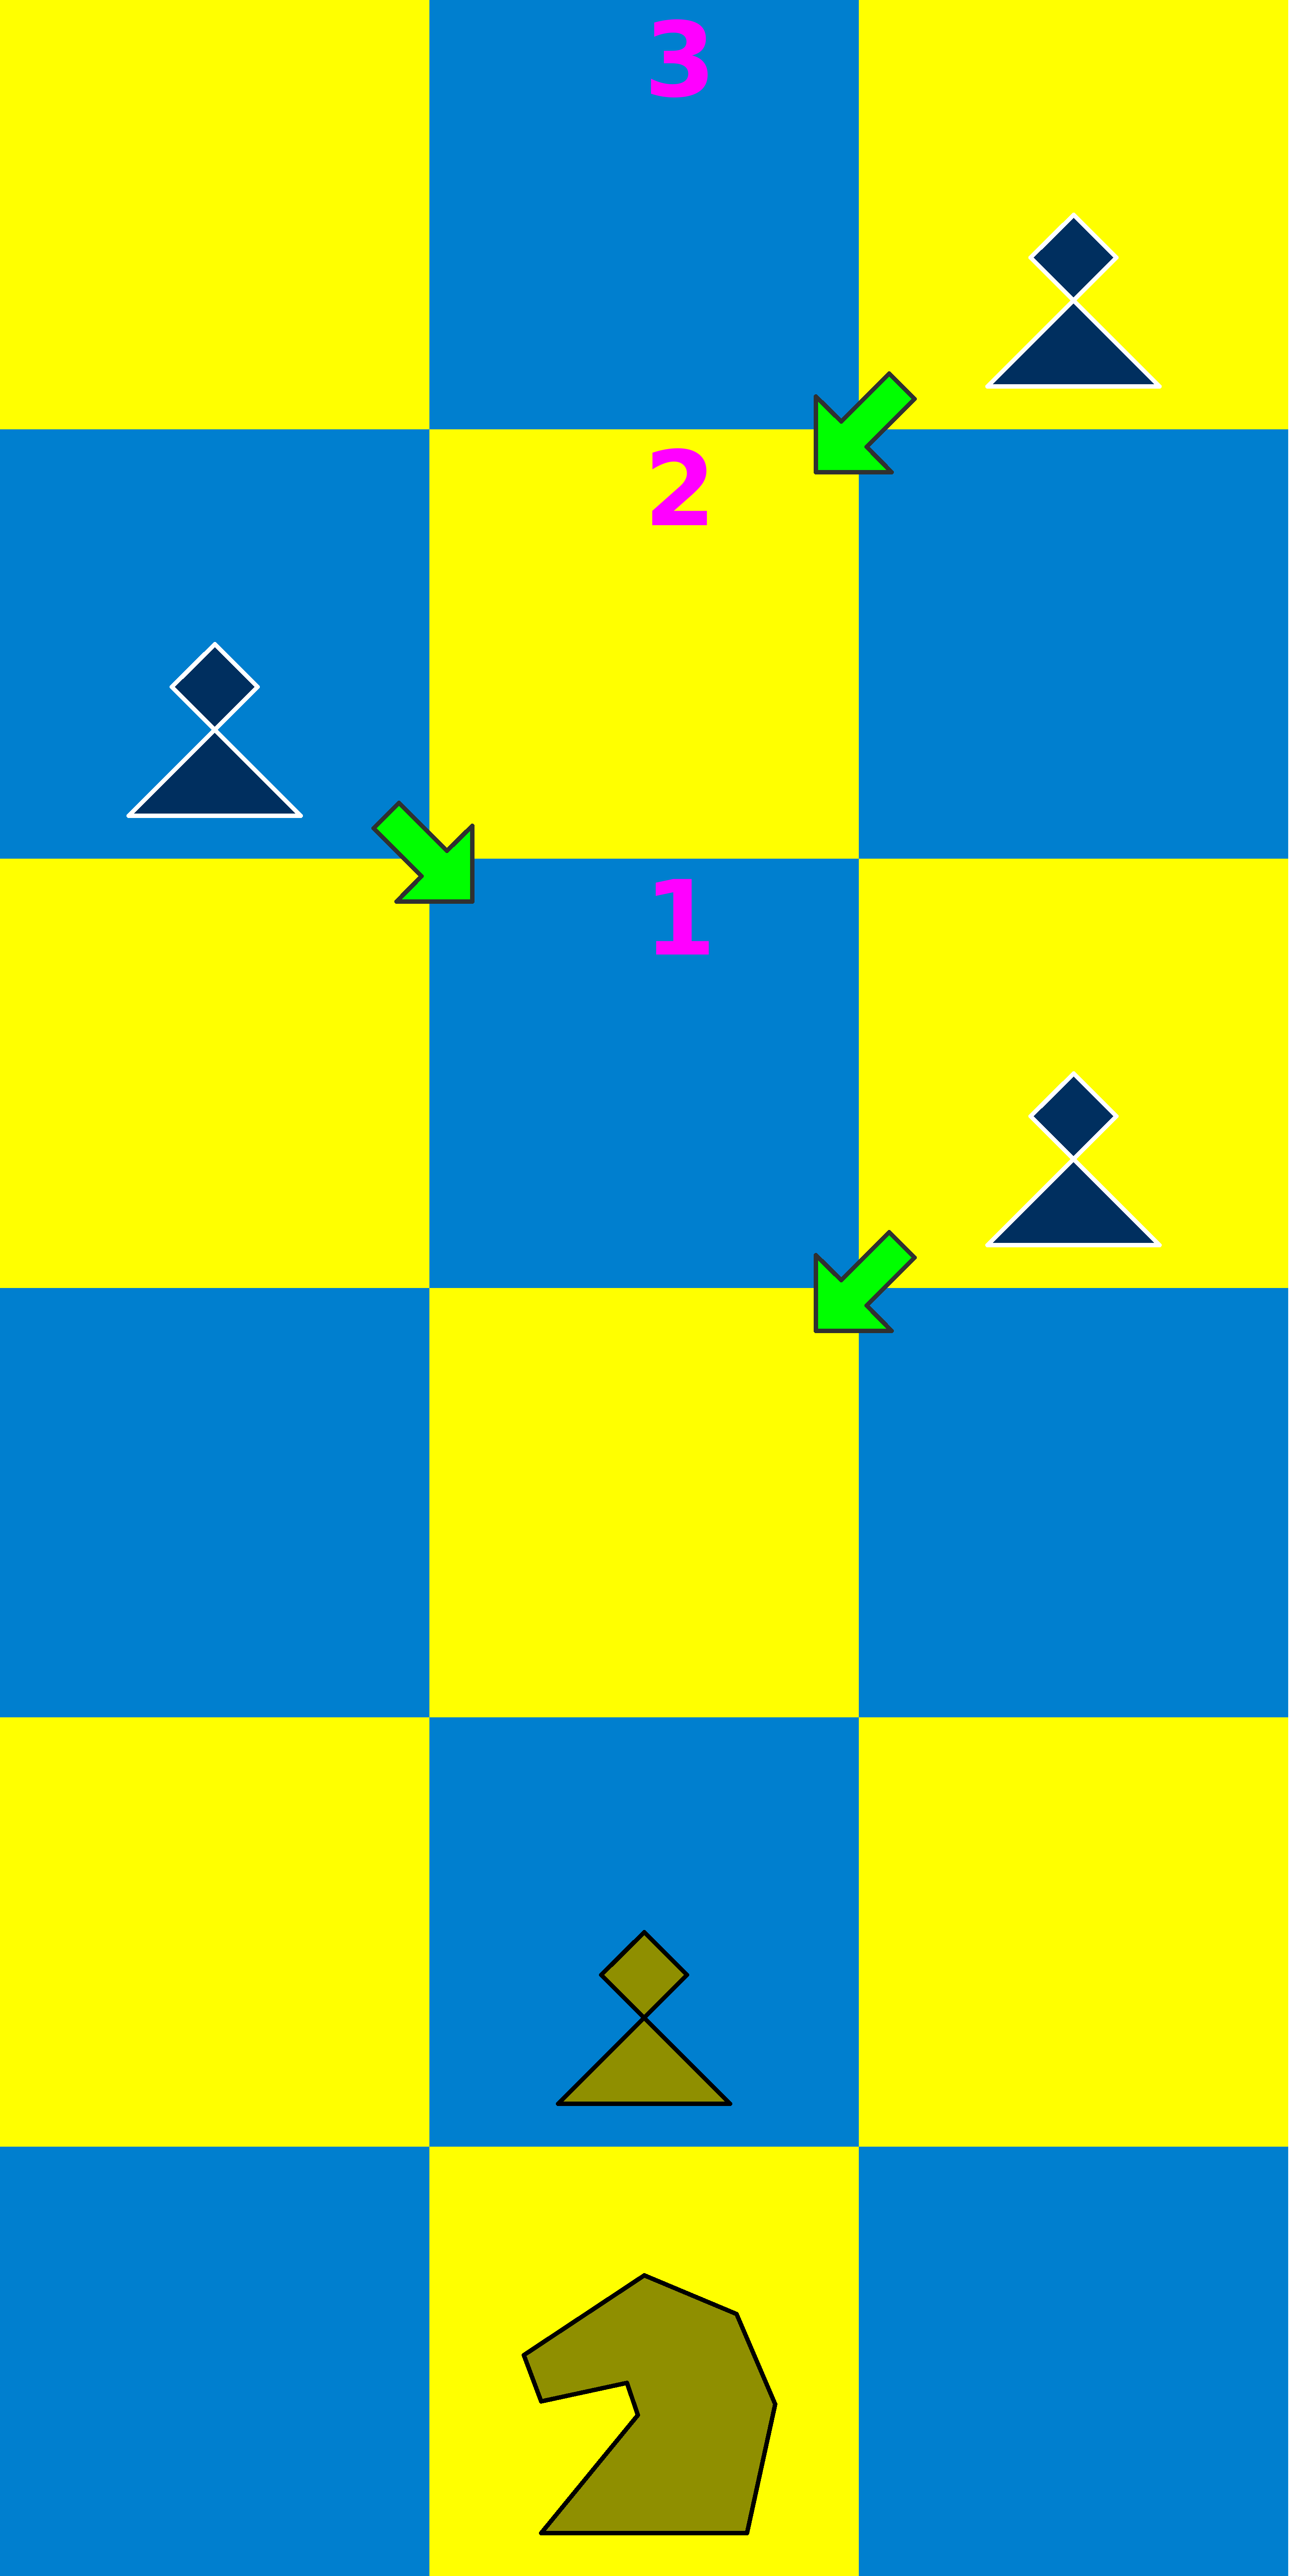
\includegraphics[width=0.25\textwidth, keepaspectratio=true]{en_passants/06_mayan_ascendancy_en_passant.png}
\caption{En passant}
\label{fig:06_mayan_ascendancy_en_passant}
\end{wrapfigure}
Rush and en passant are identical to those in Classic Chess, only difference
is that Pawn can now move longer on initial turn, up to 4 fields in this
variant.

\clearpage % ..........................................................

\section*{Castling}
\addcontentsline{toc}{section}{Castling}

Castling is essentially the same as it is in Classical Chess, only real difference is that
King can move 2, 3 or 4 fields across. All other constraints from Classical Chess still
applies.

\noindent
\begin{figure}[!h]
% \begin{figure}[!t]
\includegraphics[width=1.0\textwidth, keepaspectratio=true]{castlings/06_ma/mayan_ascendancy_castling.png}
\caption{Castling}
\label{fig:mayan_ascendancy_castling}
% \centering
\end{figure}

In example above, all valid King's castling moves are numbered. Regardless if King performs
long or short castling move, Rook would always end up on the opposite side of King on the
field immediately next to it, i.e. closer to center.

\noindent
\begin{figure}[!h]
% \begin{figure}[!t]
\includegraphics[width=1.0\textwidth, keepaspectratio=true]{castlings/06_ma/mayan_ascendancy_castling_right_03.png}
\caption{Castling long right}
\label{fig:mayan_ascendancy_castling_right_03}
% \centering
\end{figure}

In this example King was castling long to the right. Initial King's position is marked with "K".
After castling is finished, right Rook ends up at field immediately on the left to the King.

\clearpage % ..........................................................

\section*{Initial setup}
\addcontentsline{toc}{section}{Initial setup}

Compared to initial setup of Croatian Ties, Pyramid is inserted between Pegasus and Knight
symmetrically, on both sides of chessboard. This can be seen in the image below:

\noindent
% \begin{figure}[t]
\begin{figure}[h]
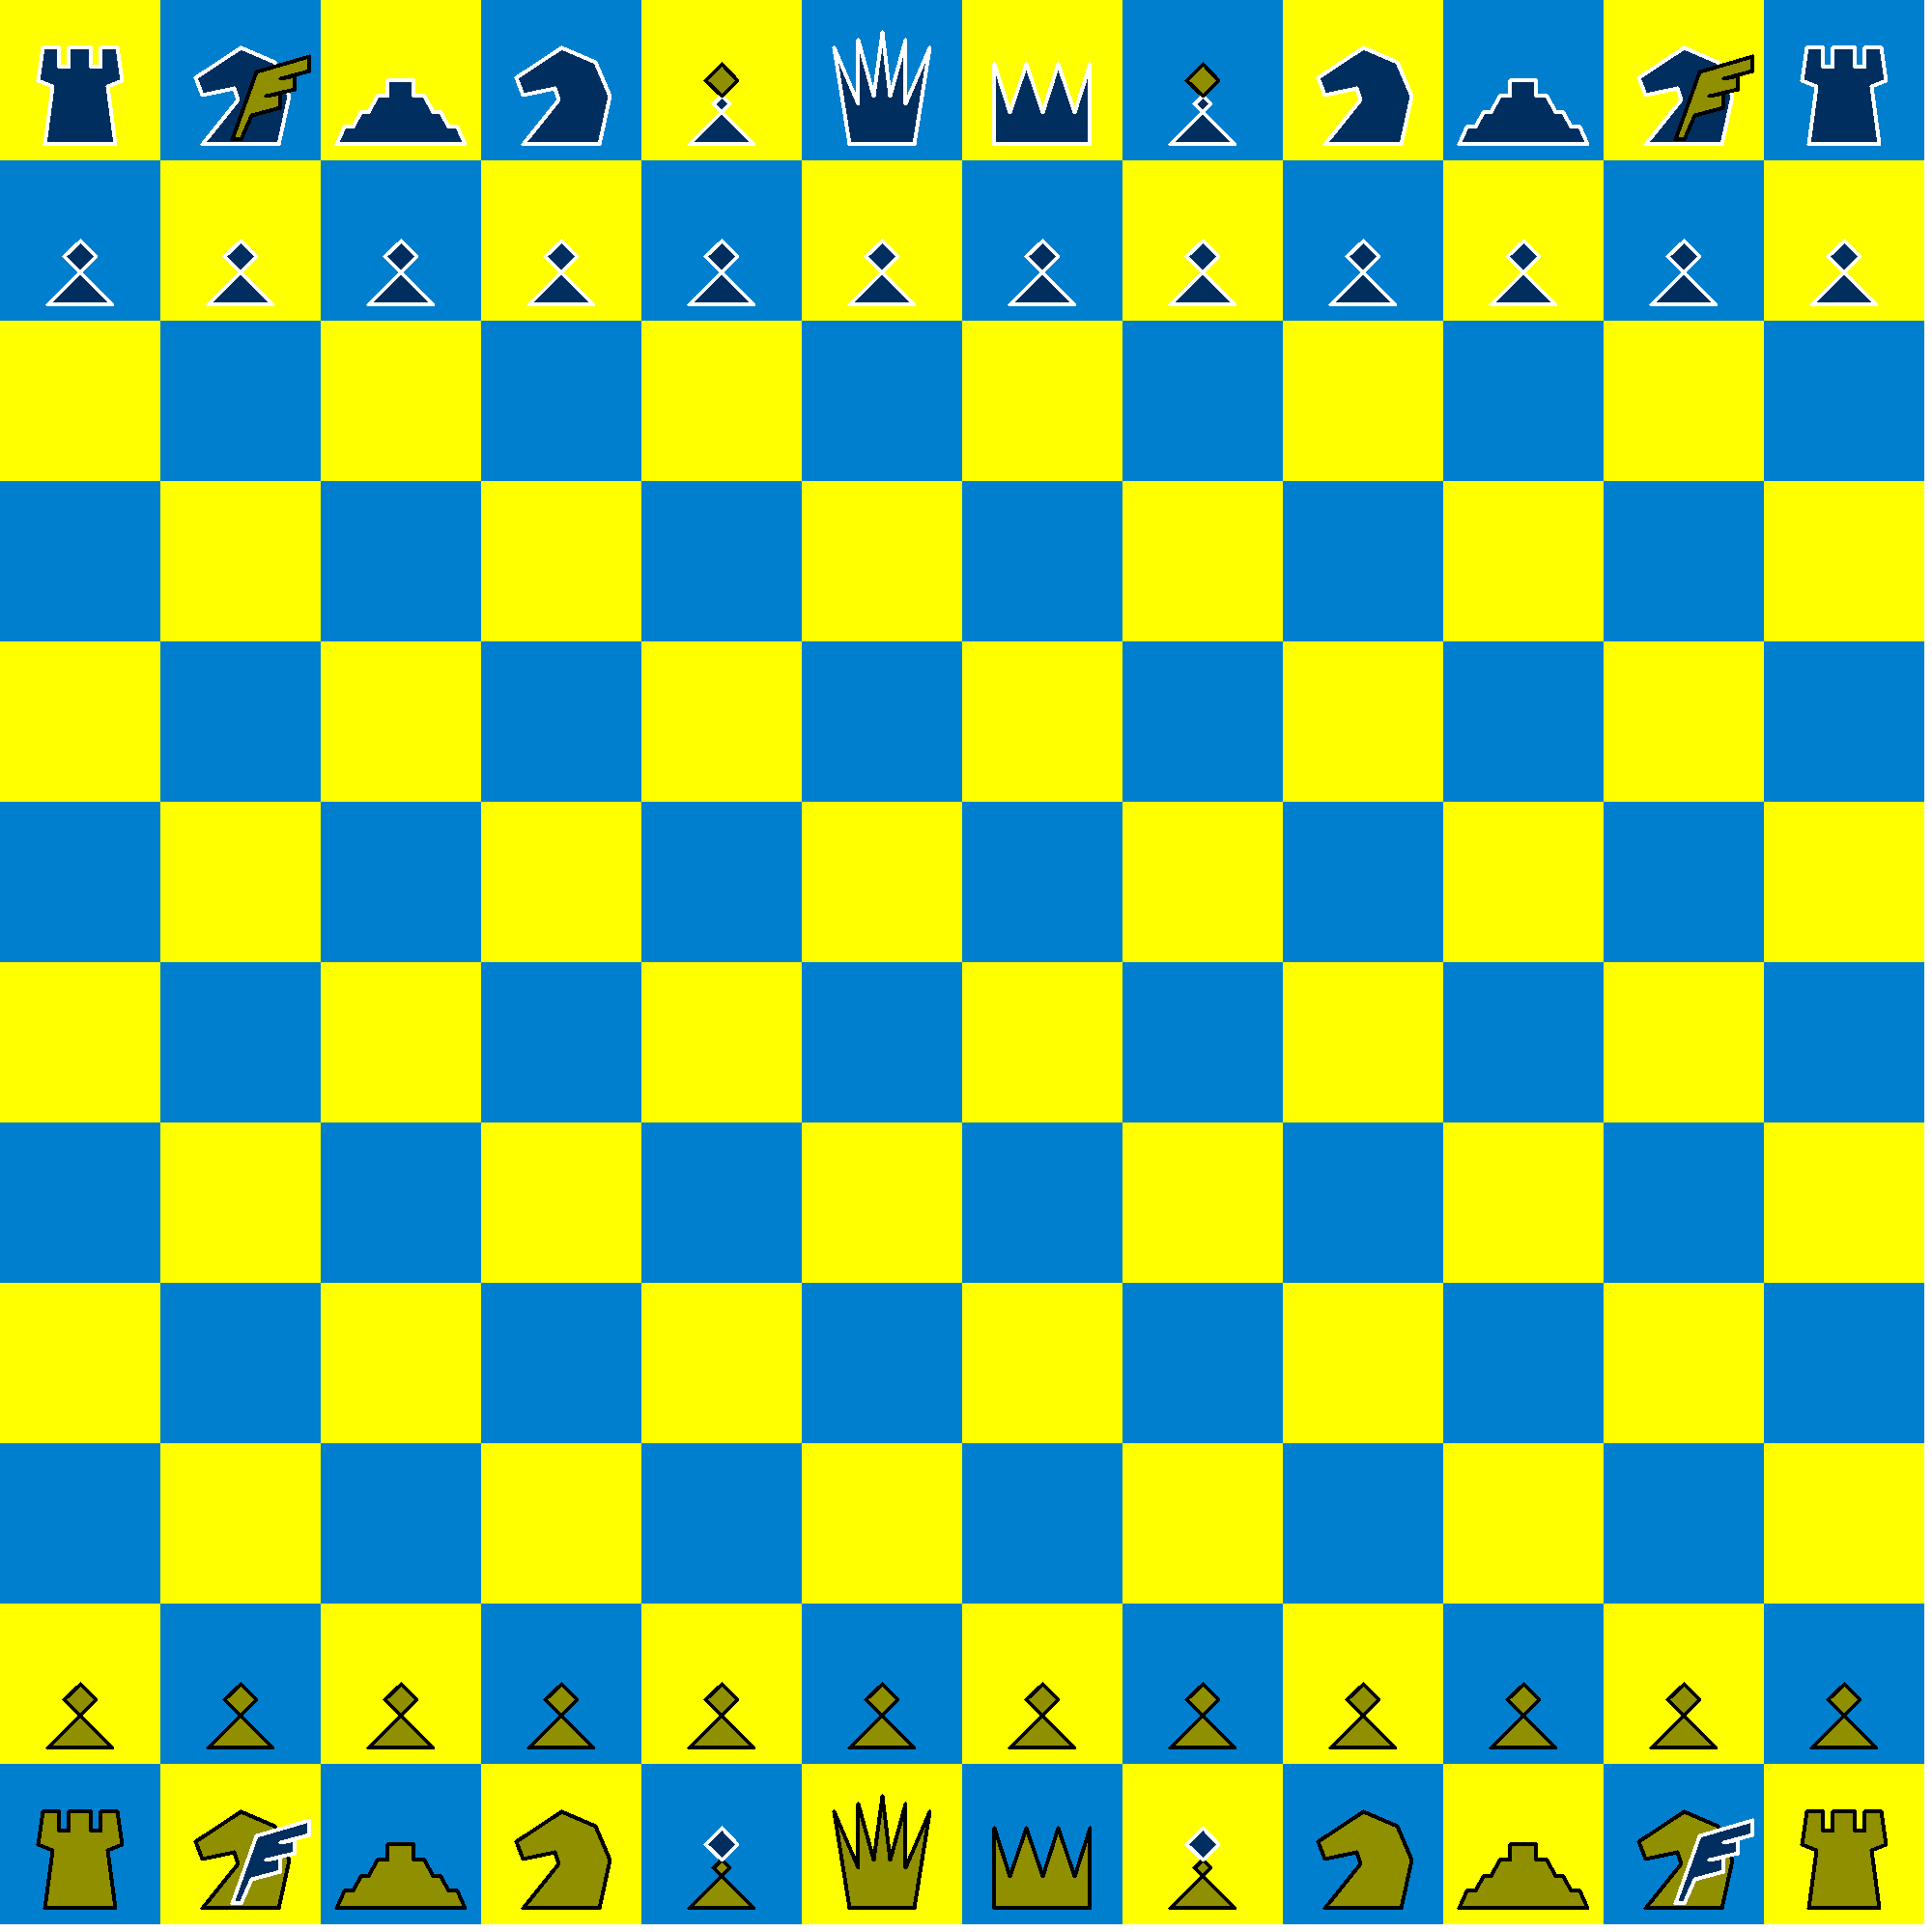
\includegraphics[width=1.0\textwidth, keepaspectratio=true]{boards/06_mayan_ascendancy.png}
\caption{Mayan Ascendancy board}
\label{fig:06_mayan_ascendancy}
% \centering
\end{figure}

\clearpage % ..........................................................
% -------------------------------------------- Mayan Ascendancy chapter
